\documentclass[12pt]{article}
\usepackage[utf8]{inputenc}
\usepackage{amssymb,amsmath,graphicx}
\usepackage[small,bf]{caption}

% add bib to ToC
\usepackage{tocbibind}

\input defs.tex

\title{Computing Market Equilibria via Convex Optimization}
\author{A.J. Friend \and Stephen Boyd}
\date{\today}

\begin{document}

\maketitle

\begin{abstract}
We consider the pure exchange market equilibrium problem of finding prices
such that the market clears, \ie, demand does not exceed supply.
This is a classic problem in economics, and has been discussed recently
in the literature from a computational complexity perspective.
Indeed, depending on the utility functions of the agents in the market,
finding equilibrium prices can be NP-hard.
This paper will focus on the numerical computation
of equilibria for a subset of markets whose equilibrium
problem can be cast as a convex program.
We introduce algorithms which scale to huge markets and can be computed
in a distributed fashion.
We report numerical results for large random markets and for
application examples in economic policy, wireless spectrum management,
and Internet advertising auctions.
\end{abstract}

\newpage
\tableofcontents
\newpage

XXX: where and how to highlight that these are exponential cone programs, and that this is something only recently efficiently solvable?

\section{Introduction}
We will consider exchange market equilibrium problems first introduced by
Walras in his in ``Elements of Pure Economics''
\cite{walras1896elements}.
Walras considers a market with agents trading
goods at prescribed prices to maximize their own utility functions.
The market equilibrium problem is that of finding prices for the goods
such that the total demand of the agents does not exceed the total amount
of each good supplied by the agents for trade.

In full generality, Walras' model includes \emph{production}, \ie, processes by which existing goods can be consumed to produce new goods which may enter the market.
We restrict this paper to the pure exchange market, which allows for trading of existing goods, but not production.

Walras suggested his natural \emph{tatonnement} price adjustment scheme as a means of computing equilibrium prices.
However, the convergence of tatonnement and conditions for existence of equilibrium prices remained an open problems for many years.

The Nobel Laureates Arrow and Debreu were the first to show that equilibrium
prices exist under mild conditions on the utility functions of agents\cite{arrow1954existence}.
However, these proofs relied on fixed-point theorems and were non-constructive.
As such, they offered no practical means by which to compute these equilibria.

This paper will investigate convex formulations of the market
equilibrium problem which were rediscovered by Jain \cite{jain2007polynomial}.
The original formulations for linear utility functions
%todo check
were stated by Nenakov and Primak \cite{nenakov1983algorithm}.
Jain's convex formulation was later extended by Chen, Ye, and Zhang \cite{chen2007note, chen2010equilibrium} to include some non-homogeneous
utility functions.

Eisenberg and Gale \cite{eisenberg1959consensus, gale1960theory, eisenberg1961aggregation} gave a convex program for a special case of Walras' model which was independently developed by Fisher. %todo citation?
This restricted case allows us to handle a larger family of utility functions
with the convex framework.

In this paper, we provide two algorithmic approaches to the convex formulations of these market equilibrium problems. The first is to use recently developed exponential cone interior point solvers to provide a centralized algorithm. The second is to use the \emph{alternating direction method of multipliers} (ADMM) \cite{boyd2011distributed} to produce a distributed and scalable algorithm, allowing us to tackle huge problems.

We provide examples and convergence results for large random markets, and 
for application examples in economic policy, wireless spectrum management,
and Internet advertising auctions.

\section{Definitions}
In this section, we give precise definitions for the market equilibrium problems that we will be studying. We define the exchange model,
which deals with agents trading initial endowments of goods to maximize their own utility functions.
A special case of the exchange model is Fisher model, where agents
start with some initial wealth, which they use to purchase goods 
from a globally available store.

\subsection{Utility functions}
The computational tractability of these problems will depend on the
utility functions of the agents in the market.
To classify these functions, we will need some simple definitions.

A function $u: \reals^n_+ \to \reals_+$ is \emph{homothetic} if for any $\alpha > 0$ we have that $u(x) \geq u(y)$ if and only if
$u(\alpha x) \geq u(\alpha y)$.
The function is \emph{monotone} or \emph{nondecreasing} if $x \geq y$ implies that $u(x) \geq u(y)$.
It is \emph{homogeneous} of degree $d$ if for any $\alpha > 0$,
$u(\alpha x) = \alpha^d u(x)$.

All the utility functions we consider in this paper will
be concave and nondecreasing.

\subsection{Exchange market}
An \emph{exchange market} has $m$ agents and $n$ goods where
agent $i$ has an initial endowment of goods $b_i \in \reals_+^n$.
Agent $i$ achieves utility $u_i(x_i) \in \reals_+$ when he is is allocated a
bundle of goods $x_i \in \reals^n_{+}$,
that is, he is allocated amount $x_{ij}$ of good $j$.

Given prices $p \in \reals^n_{++}$ for the goods, agent $i$ will sell his
initial bundle of goods, $b_i$, and buy a bundle of goods
$x_i$ to maximize his utility.
That is, agent $i$ solves the \emph{exchange utility maximization problem} (exchange UMP)
\begin{equation}
\label{p-ump}
\begin{array}{ll}
\mbox{maximize} & u_i(x_i) \\
\mbox{subject to} & p^T x_i \leq p^T b_i \\
& x_i \geq 0,
\end{array}
\end{equation}
with optimization variable $x_i$. Note that for fixed prices, $p$, the exchange UMP is a convex optimization problem.

When it won't be confused with the optimization variable,
we will denote the \emph{set} of solutions to the exchange UMP as $x^\star_i(p)$,
and refer to it as the \emph{demand} of agent $i$ at prices $p$.
Formally, $x_i^\star : \reals^n_{++} \to 2^{\reals^n_+}$ is a
\emph{relation}, \emph{set-valued mapping}, or \emph{correspondence}.
When the optimal bundle is unique, we may think of
the demand as a \emph{function}.

The \emph{exchange market equilibrium problem} (exchange MEP) is to find prices $p$ and endowments $x_i$
such that the demand for goods in the market does not exceed the supply
provided by the initial agent endowments.
The exchange model is also referred to as the Walras model \cite{walras1896elements},
the pure exchange model, or the Arrow-Debreu model.

We can write the exchange MEP as the feasibility problem
\begin{equation}
\label{p-mep}
\begin{array}{ll}
\mbox{find} & p, x_1, \ldots, x_m \\
\mbox{subject to} & x_i \in x_i^\star(p),\quad i = 1,\ldots, m \\
& \sum_{i=1}^m x_i \leq B,
\end{array}
\end{equation}
where $B = \sum_{i=1}^m b_i$ is the vector giving the total amount of each good
available for trade.


\paragraph{Tractability}
In general, however, the exchange MEP is not convex.
The computational tractability of the exchange MEP
(and the forthcoming Fisher MEP) depends on the utility functions of
the agents in the market.
For example, for general concave and increasing utility functions,
the exchange MEP is NP-hard. %todo citation
We will restrict our consideration in this paper to a subset of utility
functions for which the exchange MEP can be modeled as a convex program.

In Section~\ref{sec:convex_form_exchange}, the exchange MEP~(\ref{p-mep})
is reformulated as a problem amenable to convex optimization.
The convexity of the problem will depend on properties of the
agents' utility functions.
The admissible functions will include linear, constant elasticity
of substitution (CES), Cobb-Douglas, and a few other utilities.
A full description of these functions will be given in Section~\ref{sec:util_funcs}.
The convex formulation given bin Section~\ref{sec:convex_form_exchange} will
be the basis for the scalable algorithm for the exchange MEP, which
we will outline in Section~\ref{sec:computation}.

%convex framework is key, two different ones, but fisher can fit
% into exchange at times... best way to explain?


\subsection{Fisher market}
% todo, where do we mention what functions we can handle?

We will also consider the Fisher market, a special case of the exchange market, where agents have an initial amount of wealth (instead of an initial endowment of goods)
to purchase goods from a store of some amount of globally available goods.


A \emph{Fisher market} has $m$ agents and $n$ goods where
agent $i$ has an initial amount of money, or wealth, $w_i \in \reals_{++}$.
The total amount of good $j$ available for purchase in the market is given by
$B_j \in \reals_{++}$.

Given good prices $p \in \reals^n_{++}$, agent $i$ uses his initial
wealth $w_i$ to buy a bundle of goods $x_i$ to maximize his utility $u_i$.
That is, agent $i$ solves the \emph{Fisher~UMP}
\begin{equation}
\label{p-fisher-ump}
\begin{array}{ll}
\mbox{maximize} & u_i(x_i) \\
\mbox{subject to} & p^T x_i \leq w_i \\
& x_i \geq 0.
\end{array}
\end{equation}

We will again use $x^\star_i(p)$ to denote the demand relation
for agent $i$, \ie, the set of solutions to the Fisher UMP~(\ref{p-fisher-ump}).

The \emph{Fisher MEP} is then identical to (\ref{p-mep}), except that we use 
the Fisher definitions for $x^\star_i(p)$ and $B$.

\paragraph{Fisher is a special case of Arrow-Debreu}
We can cast any Fisher equilibrium problem as an exchange market problem using the following transformation.

Let $w_i$ be the wealth of agent $i$ and $B$ be the total amount of goods in
the Fisher system.
Let $W = \sum_{i=1}^m w_i$ be the total wealth in the Fisher market.
To form the exchange market corresponding to the Fisher system, assign an initial bundle of goods
$b_i = B w_i/W$ to agent $i$.
Since the scaling of $p$ in the exchange problem is arbitrary,
this gives the correct proportion of wealth to each agent with the correct
total amount of goods in the market.


\paragraph{Tractability}
As the Fisher problem is a special case of the exchange problem,
if the agents' utilities are compatible, we can use the convex model for the
exchange problem
to be given in Section~\ref{sec:convex_form_exchange} to solve
the Fisher MEP.

However, the Fisher problem will also admit a different
convex model to be given in Section~\ref{sec:convex_form_fisher},
which will extend the class of compatible utility functions
to those which are homogeneous of degree 1.
In particular, the Fisher MEP with Leontief utility functions
will be tractable as a convex problem, while the exchange MEP
with Leonteif utilities is NP-hard.
The compatible utility functions will be covered more completely
in Section~\ref{sec:util_funcs}.

While the convex models covered in Section~\ref{sec:convex_form} are different,
they are sufficiently similar that they will both fall under the computational
framework given in Section~\ref{sec:computation}.


\section{Convex optimization formulations}
\label{sec:convex_form}
In this section, we cover the convex formulations which can be used to solve
the Fisher and exchange market equilibrium problems.

\subsection{Exchange}
\label{sec:convex_form_exchange}
Following the formulations given in \cite{jain2007polynomial, chen2007note, nenakov1983algorithm}, it can be shown that the optimality conditions for 
the exchange MEP are equivalent to the conditions
\[
\begin{array}{ll}
& \nabla u_i(x_i)^T x_i \geq  \nabla_j u_i(x_i) \sum_k b_{ik} \frac{p_k}{p_j}, \quad \forall i,j\\
& \sum_i x_{ij} \leq \sum_i b_{ij},\quad \forall j\\
& x_{ij} \geq 0, p_j \geq 0.
\end{array}
\]
For a proof of this equivalence, see Appendix~\ref{sec:exchange_proof}.

To obtain a convex program, we first apply some transformations to the
problem.
Specifically, let $p_j = \exp(\phi_j)$, and take the logarithm of
the first set of constraints.

We obtain the optimization problem %todo fix typesetting
\begin{equation}
\label{p-exchange}
\begin{array}{ll}
\mbox{find} & x, \phi \\
\mbox{subject to} & \log(\nabla u_i(x_i)^T x_i) - \log(\nabla_j u_i(x_i)) + \phi_j 
\geq \log(\sum_k b_{ik} e^{\phi_k}),\quad \forall i,j\\
& \sum_i x_{ij} \leq \sum_i b_{ij},\quad \forall j\\
& x_{ij} \geq 0.
\end{array}
\end{equation}

Note that the optimization problem is convex if all the utility functions
in the market are such that the term
\begin{equation}
\label{e-util-constraint}
\log(\nabla u_i(x_i)^T x_i) - \log(\nabla_j u_i(x_i))
\end{equation}
is concave for all $i$ and $j$.

Note that the first constraint in (\ref{p-exchange}) need only be explicitly formed when
$\nabla_j u_i(x_i) > 0$, and we only need to include terms in the sum in
$\log(\sum_k b_{ik} e^{\phi_k})$ when $b_{ik} > 0$.
These ideas will be used later when we exploit sparsity to solve these
problems efficiently.

\subsection{Fisher}
\label{sec:convex_form_fisher}

When the utility functions are concave and homogeneous of degree 1,
the Fisher MEP is solved by the convex program
\begin{equation}
\label{p-fisher}
\begin{array}{ll}
\mbox{maximize} & \sum_{i=1}^m w_i \log u_i(x_i) \\
\mbox{subject to} & \sum_{i=1}^m x_i \leq B\\
& x_i \geq 0\quad \forall i,
\end{array}
\end{equation}
originally given by \cite{eisenberg1959consensus, gale1960theory, eisenberg1961aggregation}.
For a proof, see Appendix~\ref{sec:fisher_proof} or \cite[\S~6.2]{nisan2007algorithmic}.

The objective in this convex program is sometimes referred to as a \emph{weighted aggregate utility}, where the weights are given by the amount
of wealth $w_i$ possessed by agent $i$.
Note that only allocations $x_i$ appear as variables in the optimization
problem.
The equilibrium prices can be recovered as dual variables.

\section{Utility functions}
\label{sec:util_funcs}

In this section, we'll describe various families of utility functions
and state whether they fit into the convex programming frameworks
for Fisher, problem~(\ref{p-fisher}), and exchange markets, problem~(\ref{p-exchange}). 
It will also
be valuable to note how the expressions associated
with the utility functions may be expressed in a disciplined
convex programming framework \cite{grant2006disciplined}.

\subsection{Linear}

Linear utility functions have the form
\[
u(x) = a^T x.
\]

The utility is compatible with the exchange problem~(\ref{p-exchange}),
since
\[
\log(\nabla u(x)^T x) - \log(\nabla_j u(x))  = \log(a^T x) - \log(a_j)
\]
is concave.

This utility is compatible with the Fisher problem~(\ref{p-fisher}), as it is homogeneous of degree 1.


\subsection{Constant elasticity of substitution}
Constant elasticity of substitution (CES) functions have the form
\[
u(x) = \left(\sum_{j=1}^n a_j x_j^\rho \right)^{1/\rho}.
\]
For $-\infty < \rho \leq 1, \rho \neq 0$, the demand is a concave and
increasing function.

It is useful to note that when $\rho = 1$, we have the linear utility function. As $\rho$ approaches $0$ and $-\infty$ we recover the Cobb-Douglas and Leonteif
utility functions in the limit. %todo check which one is which

This utility is compatible with Fisher convex formulation, as it is concave and homogeneous of degree 1.

For the exchange formulation, some algebra shows that 
\begin{align*}
\log(\nabla u(x)^T x) - \log(\nabla_j u(x)) =
\log\left(\sum_{k=1}^n a_k x_k^\rho \right) - \log a_j + (1-\rho) \log x_j,
\end{align*}
which is only concave when $0 < \rho \leq 1$.

Codenotti and McCune \cite{codenotti2005marketCES} were able to provide a convex formulation which accommodated
CES functions with $-1 \leq \rho < 0$.

\subsection{Cobb-Douglas}
The Cobb-Douglas utility has the form
\[
u(x) = \prod_{j=1}^{n} x_j^{a_j},
\]
where $\sum_j a_j = 1$.


The utility is concave and homogeneous, so it is compatible with the Fisher
convex formulation.

For the exchange formulation, we have that
\begin{align*}
\log(\nabla u(x)^T x) - \log(\nabla_j u(x)) =
\log x_j - \log a_j,
\end{align*}
which is indeed concave, so the utility is also compatible with
problem~(\ref{p-exchange}).

\subsection{Leontief}
The Leontief utility has the form
\[
u(x) = \min_j a_j x_j,
\]
with $a_j \geq 0$ for each $j$. 

This utility is compatible with the Fisher formulation, as it is homogeneous and concave.

The Leontief utility is not compatible with the exchange formulation,
because the expression~(\ref{e-util-constraint}) is not concave.
In fact, this utility allows for multiple disconnected equilibria in the exchange problem. %todo cite

\subsection{Piecewise linear concave}
Piecewise linear concave functions generalize the Leontief utility, having the form
\[
u(x) = \min_k\lbrace a^{kT}x \rbrace,\quad a^k \geq 0.
\]
Just as with the Leonteif utility, they are compatible with the Fisher
formulation, but not the exchange formulation.

\subsection{Fractional power}
The fractional power function
\[
u(x) = \sum_{j=1}^n a_j (x_j+ c_j)^{d_j},
\]
where $a_j, c_j \geq 0$ and $0 \leq d_j \leq 1$,
generalizes the linear and CES utility functions.
However, these utilities need not be homothetic or homogeneous.
For example, consider $u(x,y) = \sqrt{x} + y$.

As these functions are generally \emph{not} homogeneous of degree 1,
they are not compatible with the Fisher formulation.
However, rather surprisingly, even though the
functions are not homogeneous or homothetic, they are
convex and are compatible with the exchange framework.
We see that
\begin{align*}
\log(\nabla u(x)^T x) - \log(\nabla_j u(x))
&= \log\left(\sum_{k=1}^n a_k d_k (x_k+c_k)^{d_k} - \frac{a_k d_k c_k}{(x_k + c_k)^{1-d_k}} \right)\\
&\quad- \log(a_j d_j) + (1-d_j)\log (x_j + c_j),
\end{align*}
which is seen to be concave, so this utility is compatible with
the exchange framework.

Note that a Fisher MEP with these utilities cannot
be solved with the Fisher framework~(\ref{p-fisher}),
but it can be solved by converting the
problem to the exchange form and using the exchange program~(\ref{p-exchange}).


\subsection{Logarithmic}
Logarithmic utilities have the form
\[
u(x) = \sum_{j=1}^n a_j \log(x_j+ c_j),
\]
where $a_j, c_j \geq 0$.
Again, these utilities are generally not homothetic or
homogeneous, so they will not work with the Fisher framework.
However, we see that 
\begin{align*}
\log(\nabla u(x)^T x) - \log(\nabla_j u(x)) =
\log\left(\sum_{k=1}^n a_k - \frac{a_k c_k}{x_k+c_k} \right) - \log a_j + \log (x_j + c_j),
\end{align*}
which is indeed concave, so the utilities are compatible
with the exchange framework.

Again, we can transform a Fisher problem with these utilities into
an exchange problem and use the exchange framework to solve
the Fisher MEP.

\section{Algorithms}
\subsection{Centralized conic programming algorithm}
\label{sec:centralized}
As the market equilibrium problems we have described are convex, one might expect that they could be easily formulated and solved with currently
available modeling frameworks and optimization solvers.
This is indeed the case, but only due to recent advances in convex solvers,
such as SCS and ECOS-Exp. %todo cite
For the first time, these solvers can handle exponential cone constraints,
which are needed to represent the logarithm and exponential functions found in 
formulations (\ref{p-exchange}) and (\ref{p-fisher}).

We can describe these market equilibrium problems easily using the modeling
framework CVXPY (XXX: cite), and solve the models using SCS. Section~\ref{sec:centralized} will give computational results for moderately sized problems. Indeed, these are the largest general market equilibrium problems we have seen solved in the literature. However, for much larger problems, we will
be limited by solving these problems in a centralized fashion. The next section will describe distributed methods which will scale to arbitrarily large problems.


\subsection{Distributed ADMM algorithm}
\label{sec:distributed}

%todo introduce prox operators?
We can compute solutions to both the Fisher and exchange convex
formulations, problems (\ref{p-fisher}) and (\ref{p-exchange}), using
the alternating direction method of multipliers (ADMM) \cite{boyd2011distributed, parikh2013proximal}.

We'll see that we can put both problems into the ADMM-compatible form
\begin{equation}
\label{p-admm}
\begin{array}{ll}
\mbox{minimize} & \sum_{i=1}^m f_i(x_i, \phi_i) \\
\mbox{subject to} & \sum_{i=1}^m x_i \leq B\\
& \phi_i = \Phi, \quad \forall i
\end{array}
\end{equation}
for appropriately chosen functions $f_i$.
Recall that the vector $B \in \reals^n_{++}$ gives the total
amount of goods available in the market. In the Fisher problem,
$B$ is given.
In the exchange problem, $B = \sum_i b_i$.
The variables $x_i$ give the local allocations for agent $i$, and
$\phi_i \in \reals^n_{++}$
are the local log-prices, which must agree globally through the
consensus variable $\Phi$.
(In the Fisher formulation, $f_i$ will not depend on $\phi$.)

In the remainder of this subsection, we describe the $f_i$ functions for the exchange and Fisher cases, and provide a general
ADMM implementation to solve either case.

\paragraph{Fisher}
We can simply assign
\[
f_i(x_i, \phi) = -w_i \log u_i(x_i) + I_{\lbrace x \mid x \geq 0 \rbrace}(x_i),
\]
where the second term is the indicator function for the positive orthant.
We see that problem~(\ref{p-admm}) is equivalent to
problem~(\ref{p-fisher}).

\paragraph{Exchange}

For agent $i$, let $f_i(x_i, \phi)$ be the indicator function for the
constraints
\[
\begin{array}{c}
\log(\nabla u_i(x_i)^T x_i) - \log(\nabla_j u_i(x_i)) + \phi_j \geq  \log\left(\sum_k b_{ik} e^{\phi_{k}}\right),\quad \forall j\\
x_i \geq 0.
\end{array}
\]
We see that problem~(\ref{p-admm}) is equivalent to problem~(\ref{p-exchange}).


\paragraph{Notation}
XXX note: The admm algorithm in this section is written for the more general case of 
the exchange problem, so it includes $\phi$ variables.
The fisher problem doesn't involve $\phi$, so it may not really make sense
to write a single algorithm for both settings. figure out later...

We can use an ADMM-based splitting method \cite{boyd2011distributed} to
solve the market equilibrium problem written in the form of
problem~(\ref{p-admm}).
We will be interested in exploiting sparsity in the market, such
as each agent only being interested buying and selling a small subset 
of all the possible goods.
For this purpose, we will use an indexing notation in this section which is
more suitable to represent this sparsity and will simplify our resulting
ADMM equations.

Let $\mathcal{G}$ be an indexing set for all goods
in the market.
Agent $i$ will purchase amount $(x_i)_g$ of good $g \in \mathcal{G}$.
(We will also write $x_{ig}$ to lighten notation.)
Agent $i$'s utility is a function of the bundle $x_i \in \reals_{+}^{|G_i|}$,
where $G_i \subset \mathcal{G}$ is the set of goods involved in the utility
function $u_i$.

Note that we don't specify the actual ordering of the elements
of the vector $x_i$, as we will just care about the values associated with
each good.
When we do any operations (such as addition or scalar product) with
two vectors corresponding to the same subset of goods, we will
assume that the operation is done in a way that respects the local ordering of
the goods.

Agent $i$ is also initially endowed with a set of goods
$H_i \subset \mathcal{G}$,
with allocation values $(b_i)_g = b_{ig}$, where $b_i \in \reals_{++}^{|H_i|}$.
Again, $B \in \reals^n_{++}$ will be the total amount of goods in the market, which, in our
current notation, we can represent as
\[
B_g = \sum\limits_{i \in H^{-1}_g} b_{ig}
\]
for each good $g \in \mathcal{G}$.

We will treat $G$ and $H$ as \emph{relations},
using subscript notation instead of function notation.
As we have seen, $G_i$ corresponds to the set of goods that agent $i$ is
interested
in possibly purchasing.
The relation notation will also allow us to
write $G^{-1}_g$ to denote the set of agents which are interested in
purchasing good $g$.
Similarly, $H^{-1}_g$ is the set of agents initially endowed with some
positive amount of good $g$.

In the ADMM algorithm, each agent will have a local opinion for the prices
of the goods he is interested in purchasing or selling.
We represent his local log-prices
by $\phi_i \in \reals_+^{|G_i \cup H_i|}$.

Note that
\[
\bigcup_{i=1}^n G_i = \bigcup_{i=1}^n H_i = \mathcal{G}.
\]

For any variable $z \in \reals^{|\mathcal{G}|}$ which contains values for
each good in the market, we may write $z_{G_i}$ to represent the subvector
of $z$ whose elements correspond to the goods in $G_i$.

\paragraph{ADMM problem form} Then the problem we'd like to solve is given by
problem (\ref{p-admm}), but we'll rewrite it here using this section's notation.
We will also replace the inequality constraint on purchased goods with an
equality, since this simplifies the ADMM iteration, and we know that
the constraint is tight at equilibrium.
The reformulated problem is
\[
\begin{array}{ll}
\mbox{minimize} & \sum_i f_i(x_i, \phi_i) \\
\mbox{subject to} & \sum\limits_{i \in G^{-1}_g} x_{ig} = B_g,\quad \forall g \in \mathcal{G}\\
& \phi_{ig} = \Phi_g,\quad \forall i \in G^{-1}_g \cup H^{-1}_g,\ \forall g \in \mathcal{G}.
\end{array}
\]

The first set of constraints are the global resource constraints; the amount of
goods purchased by agents cannot exceed the total initial endowed amount.
The second set of constraints are consensus constraints on the price variables,
$\phi_i$.
Each agent will have an opinion on the price of a good if he is buying or selling it.
The constraint says that all agents with an opinion, $\phi_{ig}$, on the price
of good $g$ must agree.
They agree through a global consensus variable $\Phi$.


\paragraph{ADMM algorithm}
Note that we have a generalized consensus problem in the price variables,
$\phi$, and a generalized sharing problem in the allocation variables, $x$.

The resulting ADMM algorithm is 
\begin{align}
\label{a-xtild}
\tilde{x}^k_g &:= \frac{1}{|G^{-1}_g|} \left( \sum_{i \in G^{-1}_g} x^k_{ig} - \sum_{i \in H^{-1}_g} b_{ig}\right)\\
\label{a-phibar}
\bar{\phi}^k_g &:= \frac{1}{ |G^{-1}_g \cup H^{-1}_g| } \sum_{i \in G^{-1}_g \cup H^{-1}_g}\phi^k_{ig}\\
u^{k+1} &:= u^k + \tilde{x}^k\\
w_i^{k+1} &:= w_i^k + \phi^k_i - \bar{\phi}^k_{G_i}\\
\label{a-prox}
x_i^{k+1}, \phi_i^{k+1} &:= \mbox{prox}_{f_i}(x_i^k - \tilde{x}^k_{G_i} - u^{k+1}_{G_i},
\bar{\phi}^k_{G_i} - w_i^{k+1}).
\end{align}

This algorithm needs to be explained.
In equation~(\ref{a-xtild}), $\tilde{x}^k_g$ gives a measure of the violation of
the global resource constraint, normalized by the number of agents participating
in considering that good.
In equation~(\ref{a-phibar}), $\bar{\phi}^k_g$ gives the average of the price
opinions $\phi^k_g$ over all agents with an interest in the price of good $g$.
Dual variables $u^k$ and $w^k_i$ are updated in the next two equations.
Note that $\tilde{x}^k$, $\bar{\phi}^k$, and $u^k$ are \emph{global} variables
and that $w_i^k$, $x_i^{k+1}$, and $\phi_i^{k+1}$ are \emph{local} variables
for each agent. In equation~(\ref{a-prox}), each agent computes the projection
onto his local optimality constraints.
The input to this proximal operator is formed by combining
local and global variables.
For example, since $\tilde{x}^k$ is a global variable with values for each good in the market, we use the notation $\tilde{x}^k_{G_i}$ to denote the subset of this vector corresponding to goods in $G_i$.
Each agent emits the results of their proximal operator and the
global computation of $\tilde{x}^{k+1}_g$ and $\bar{\phi}^{k+1}_g$ continues in the next step.

The algorithm above is decentralized and parallelizable.
Each agent can compute their prox operator separately and in parallel.
The results of these prox operators are aggregated, averaged, and then distributed
back to the individual agents for the next iteration.





\section{Examples}
\subsection{Random problem data generation}
\label{sec:random_prob}
We will generate random exchange market instances to test our algorithms.
We describe the generation procedure here.
The random markets in these tests will be parameterized
by a single number, $n$, which will be both the
number of agents and the number of goods in the market.

Each agent will have a utility function involving $r = \min(n,20)$
goods.
We choose this set of goods for each agent by randomly selecting
$r$ distinct goods from the pool of $n$ possible goods.
The utility function of the agent has an equal chance of 
being either of the fractional power or logarithmic form.
The parameters for the utility functions, $a_i$, $c_i$, and possibly
$d_i$ will be drawn from a uniform distribution on $[0,1]$ for each good.
Note that the fractional power and logarithmic utilities include
linear, CES, and Cobb-Douglas utilities as special cases,
so we consider this family of random utilities to be reasonably general.

Each agent will also be endowed with nonzero amounts of $r$
goods.
The set of $r$ goods will again be drawn from the pool of $n$
without replacement, and the initial endowment of
the resulting goods will be drawn from a uniform distribution on
$[0,1]$.

To ensure that equilibrium prices are meaningful and non-trivial,
we will assign the random subsets of goods for utility functions and
initial endowments in such a way that every good is desired by at least one agent, and every good is provided by at least one agent.

\subsection{Relative residuals}
To evaluate our computational experiments, we propose a measure of
the relative \emph{dissatisfaction} of an agent in a market, given
market log-prices $\Phi$ and an algorithmically-prescribed bundle of goods
$x$.
That is, for any bundle of goods and proposed log-prices, we will compare the
utility assigned to an agent via its assigned bundle with the maximum utility
the agent could acheive by solving his UMP at the given prices.

For agent $i$, with prescribed bundle $x_i$ and global log-prices $\Phi$,
we define the relative residual to be
\[
q_i(x_i, \Phi)= \max\left(0,1-\frac{u_i(x_i^k)}{u_i(x_i^\star(\Phi^k))}\right).
\]
Note that $q_i \in [0,1]$ is a measure of the dissatisfaction of agent $i$.
If the agent is assigned more utility (by violating his spending constraints) than he would get by solving his UMP, he has $q_i = 0$ dissatisfaction.
On the other hand, if, at the given prices, he has $q_i = .03$, for instance, then he has only been assigned $97\%$ of his maximum possibe utility (at the given prices).

Using the relative residual as a measure of convergence for our iterative ADMM
algorithm only makes sense if we project a proposed solution onto positivity and
global resource availability constraints. Otherwise, we could assign each agent an arbitrarily large bundle of goods and acheive 0 dissatisfaction.
Thus, in the experiements below, at each ADMM iterate, we will transform the iterate $x_i^k$ so that the assignments are positive, and their sum does not violate the global allocation constraint.

In the experimental results given, we will plot both the worst-case nd average relative residual (both taken over all the agents in the market).

\subsection{Centralized algorithm}
To demonstrate the centralized algorithm of Section~\ref{sec:centralized},
%todo add SCS section, fix section reference
we generate random exchange markets ranging in size
from $n=10^1$ to $n=10^3$.
For each problem size, we generate 10 market instances to demonstrate
variance in solve time.
Figure~(\ref{f-cvxpy}) %todo fix
plots the SCS solve time as a function of problem size, running
SCS on its default parameters, with a stopping tolerance of $10^{-3}$,
running on a 2013 macbook air, with 8 gb ram and a 1.7 GHz processor.
The same figure also provides the average and worst case relative residual over the agents of the market.


\begin{figure}
\begin{center}
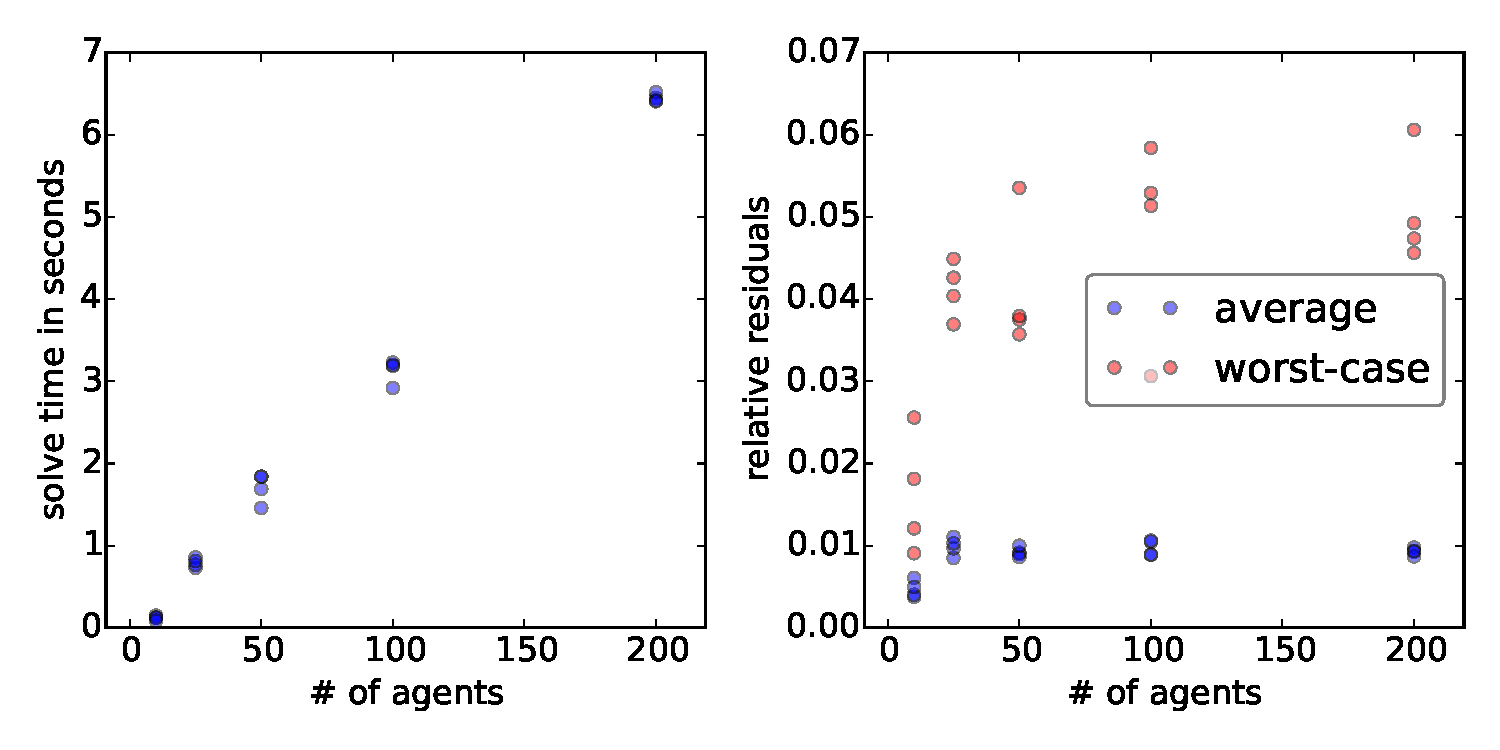
\includegraphics[width=1.0\textwidth]{figures/cvxpy}
\caption{XXX temporary figure. For different values of numbers of agents, $n$,
we generate 10 random instances of a market, as in Section~\ref{sec:random_prob}. We solve each market problem with the centralized method, using SCS, and report the solve times and average and worst-case relative residuals, with the statistics taken over the agents in the market, not market instances.}
\end{center}
\label{f-cvxpy}
\end{figure}


\subsection{Decentralized algorithm}
To demonstrate our decentralized algorithm of Section~\ref{sec:distributed},
%todo fix section ref
we solve a single random instance of size $n=10^6$ agents.
At each iteration, we take the result of the prox operation (\ref{a-prox}) and the consensus prices $\Phi^k$ from (\ref{a-phibar}) and compute
the average and worst-case relative residual over the agents in the market
and record the findings
in Figure~(\ref{f-admm}) %todo figure ref.

\begin{figure}
\begin{center}
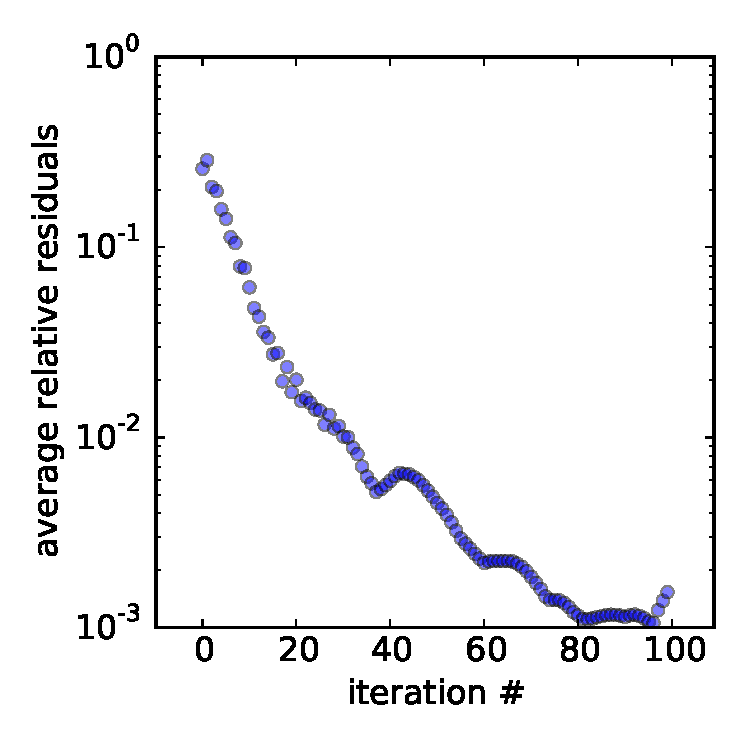
\includegraphics[width=0.6\textwidth]{figures/admm}
\caption{XXX temporary figure. This figure gives results for decentralized ADMM algorithm applied to a single random market generated as in Section~\ref{sec:random_prob} with $n=10$ agents. We give the average and worst-case statistics of the agents for their relative residuals.}
\end{center}
\label{f-admm}
\end{figure}



\section{Applications}
\cite{shoven1992applying}

see \cite{shoven1992applying} for examples and applications of nested CES functions

\begin{itemize}
\item traffic
\item routing
\item spectrum management
\item others?
\end{itemize}

\appendix




\section{Convex formulation for exchange}
\label{sec:exchange_proof}
The primal Arrow-Debreu problem has the form
\[
\begin{array}{ll}
\mbox{minimize} & - u_i(x_i)\\
\mbox{subject to} & p^T x_i \leq p^T b_i\\
& x_i \geq 0.
\end{array}
\]

The dual problem has the form
\[
\begin{array}{ll}
\mbox{maximize} & -(- u_i)^*(\tau_i - p y_i) - p^T b_i y_i\\
\mbox{subject to} & y_i \geq 0\\
& \tau_i \geq 0.
\end{array}
\]

We can also write down the optimality conditions for the equilibrium allocation,
which includes a global resource constraint.

\begin{align*}
-\nabla u_i(x_i) + p y_i &= \tau_i\\
y_i p^T x_i &= y_i p^T b_i \\
\tau_i^T x_i &= 0\\
p^T x_i &\leq p^T b_i\\
x_i, y_i, \tau_i &\geq 0\\
\sum_{i} x_{ij} &\leq \sum_{i} b_{ij}
\end{align*}

First, we'll simplify the constraints by removing $\tau$:

\begin{align*}
p y_i &\geq \nabla u_i(x_i) \\
y_i p^T x_i &= y_i p^T b_i \\
y_i p^T x_i &= \nabla u_i(x_i)^T x_i\\
p^T x_i &\leq p^T b_i\\
x_i, y_i &\geq 0\\
\sum_{i} x_{ij} &\leq \sum_{i} b_{ij}
\end{align*}

Next, we remove the $y$ variables by combining the second and third constraint
to get that
\[
y_i = \frac{\nabla u_i(x_i)^T x_i}{p^T b_i},
\]
and plug it into the first constraint to get the new set of constraints:
\begin{align*}
\frac{\nabla u_i(x_i)^T x_i}{p^T b_i} p &\geq \nabla u_i(x_i) \\
p^T x_i &\leq p^T b_i\\
x_i, y_i &\geq 0\\
\sum_{i} x_{ij} &\leq \sum_{i} b_{ij}.
\end{align*}

We'll drop the second constraint, as it is implied by the others:
\begin{align*}
\nabla u_i(x_i)^T x_i p_j &\geq \nabla_j u_i(x_i) p^T b_i\quad \forall i,j \\
\sum_{i} x_{ij} &\leq \sum_{i} b_{ij}\quad \forall i\\
p, x_i &\geq 0\quad \forall i.
\end{align*}

\paragraph{Equivalence with original constraints}
To see the equivalence with the original constraints, take the first inequality,
multiply by $x_{ij}$ and sum over $j$ to get
\begin{align*}
\sum_j \nabla u_i(x_i)^T x_i p_j x_{ij} &\geq \sum_j \nabla_j u_i(x_i) x_{ij} p^T b_i \\
\implies \nabla u_i(x_i)^T x_i p^T x_i &\geq \nabla u_i(x_i)^T x_i p^T b_i \\
\implies p^T x_i &\geq p^T b_i.
\end{align*}

Note that the last constraint implies that
\[
p_j \sum_i x_{ij} \leq p_j \sum_i b_{ij}.
\]

Now, we have that

\begin{align*}
\sum_i p^T b_i &\leq \sum_i p^T x_i\quad \text{(by something)}\\
&= \sum_j p_j \sum_i x_{ij} \\
&\leq \sum_j p_j \sum_i b_{ij}\quad \text{(by something)}\\
&= \sum_i p^T b_i.
\end{align*}

This implies equality holds throughout, so, in particular,
\begin{align*}
p^T x_i &= p^T b_i\\
\sum_i x_{ij} &= \sum_i b_{ij}
\end{align*}

This recovers all the original constraints.

\section{Convex formulation for Fisher}
\label{sec:fisher_proof}
We prove that solutions to the convex formulation %todo ref
are indeed equilibrium allocations.


\section{Other solution methods}
XXX: some ideas to pursue in the future

\subsection{Infinite LP/cutting plane methods}
That WGS gives a cutting plane is proved in \cite{arrow1959stability}.
(supposedly... check, as the papers have similar names.)

\subsection{Tatonnement}

\subsection{Weighted total utility}
put in the fisher stuff here. arrow-debreu can be solved this way, but we
don't know the weights. introduce re-weighting idea.

\subsection{CVXPY and SCS}

\subsection{Monotone operators}
For many utility functions,
%todo when?
the excess demand function
(or correspondence,
or relation) of an agent is a
monotone operator.
That is,
\begin{equation}
\label{e-monotone}
\left[z(p) - z(q) \right]^T \left[p - q\right] \leq 0.
\end{equation}

If we assume that Walras' Law holds, \ie, each agent spends their entire
budget, or $p^T z(p) = p^T x(p) - p^T b = 0$, then the operator monotonicity has
a nice economic interpretation in terms of \emph{preferences}.

Expanding inequality~(\ref{e-monotone}) and applying Walras' Law, we find that
\[
p^T z(q) + q^T z(p) \geq 0.
\]

We thus see that the implication
\begin{equation}
\label{e-preference}
p^T z(q) \leq 0 \implies q^T z(p) \geq 0
\end{equation}
is equivalent
%todo or just implies? is it actually true that they are equivalent?
to inequality~(\ref{e-monotone}) whenever Walras' Law holds.

We interpret (\ref{e-preference}) as revealing that the agent prefers prices
$p$ over prices $q$. If $p^T z(q) \leq 0$, then $p^T x(q) \leq p^T b$, implying
that both bundles $x(p)$ and $x(q)$ are affordable (feasible) at prices $p$.
Since $x(p)$ is an optimal bundle at prices $p$, we know that it must be at least
as preferred at $x(q)$, or that $u(x(p)) \geq u(x(q))$.

Inequality~(\ref{e-monotone}) already shows that implication~(\ref{e-preference})
holds, but to interpret the result economically, suppose that the
implication did not hold, \ie, that $q^T z(p) < 0$. We would then have that
$q^T x(p) < q^T b$, which implies that $x(p)$ and $x(q)$ are both affordable
bundles at at prices $q$. However, we know that $u(x(p)) \geq u(x(q))$, so
bundle $x(p)$ must be optimal, and Walras' Law implies $q^T x(p) = q^T b$, which
gives a contradiction. 

In the case of strict inequality, if $p^T z(q) < 0$, then $q^T z(p) > 0$.
That is, $x(p)$ is revealed as preferred to $x(q)$, and $x(p)$ is not within
budget at prices $q$, so prices $p$ are preferred by the agent.

Note that if each agent's excess demand function is a monotone operator, then
the market's aggregate excess demand function is also monotone. If these
operators are \emph{maximal} monotone, then we can use the this framework for
solving these problems.
%todo However, it is unclear if and when these operators are maximal.

Even in the case that the operators are monotone but not maximal, we still get
a cutting-plane by computing the demand function. That is, for any prices $p$
and optimal prices $p^*$, we have that
\[
p^{*T} z(p) \geq 0,
\]
which gives us a cutting-plane in the price simplex.
A cutting-plane algorithm can then be used to compute the optimal prices

\paragraph{Computing the resolvent}
The resolvent of the excess demand operator is
\[
(I + \lambda z)^{-1}(p) = q,
\]
which we parse to interpret as
\[
p = q + \lambda x(q) - \lambda b.
\]
That is, given prices $p$, we must find prices $q$ such that the agent's UMP
at prices $q$ satisfy the above quality.

XXX: We can write down the optimality conditions, but these may put the same
constraints on the utility functions as the Ye formulation. We can always
substitute $p = q + \lambda x(q)$ into the opt conditions to remove either
$q$ or $x$. But we end up with a non-convex problem. We optimize over the a
non-convex region, something like the space outside of a unit ball.
We may also be able to formulate the problem as being bi-convex in $x$ and $q$,
but I'm not sure how helpful that would be.

\subsection{Cutting plane}
\paragraph{Approximations?}
can i approximate the exponential cone to do an approximate prox evaluation
at each step, allowing for SOCP solvers that can't handle exponential cones?

what if we approximate everything with a quadratic around the current iterate
for an approximate projection? subset or superset of actual agent cutting set?
does this simplification make updates with an analytic form, allowing for very
fast iteration?



\newpage
\bibliographystyle{alpha}
\bibliography{bibliography}

\end{document}


